%!TEX root = ../diffusion_paper.tex
\section{Results} % (fold)
\label{sec:results}
  \subsection{TDS on Synthetic Geometries} % (fold)
  \label{sub:tds_on_synthetic_geometries}
  \begin{figure}[!t]
    \centering
    \subfloat[]{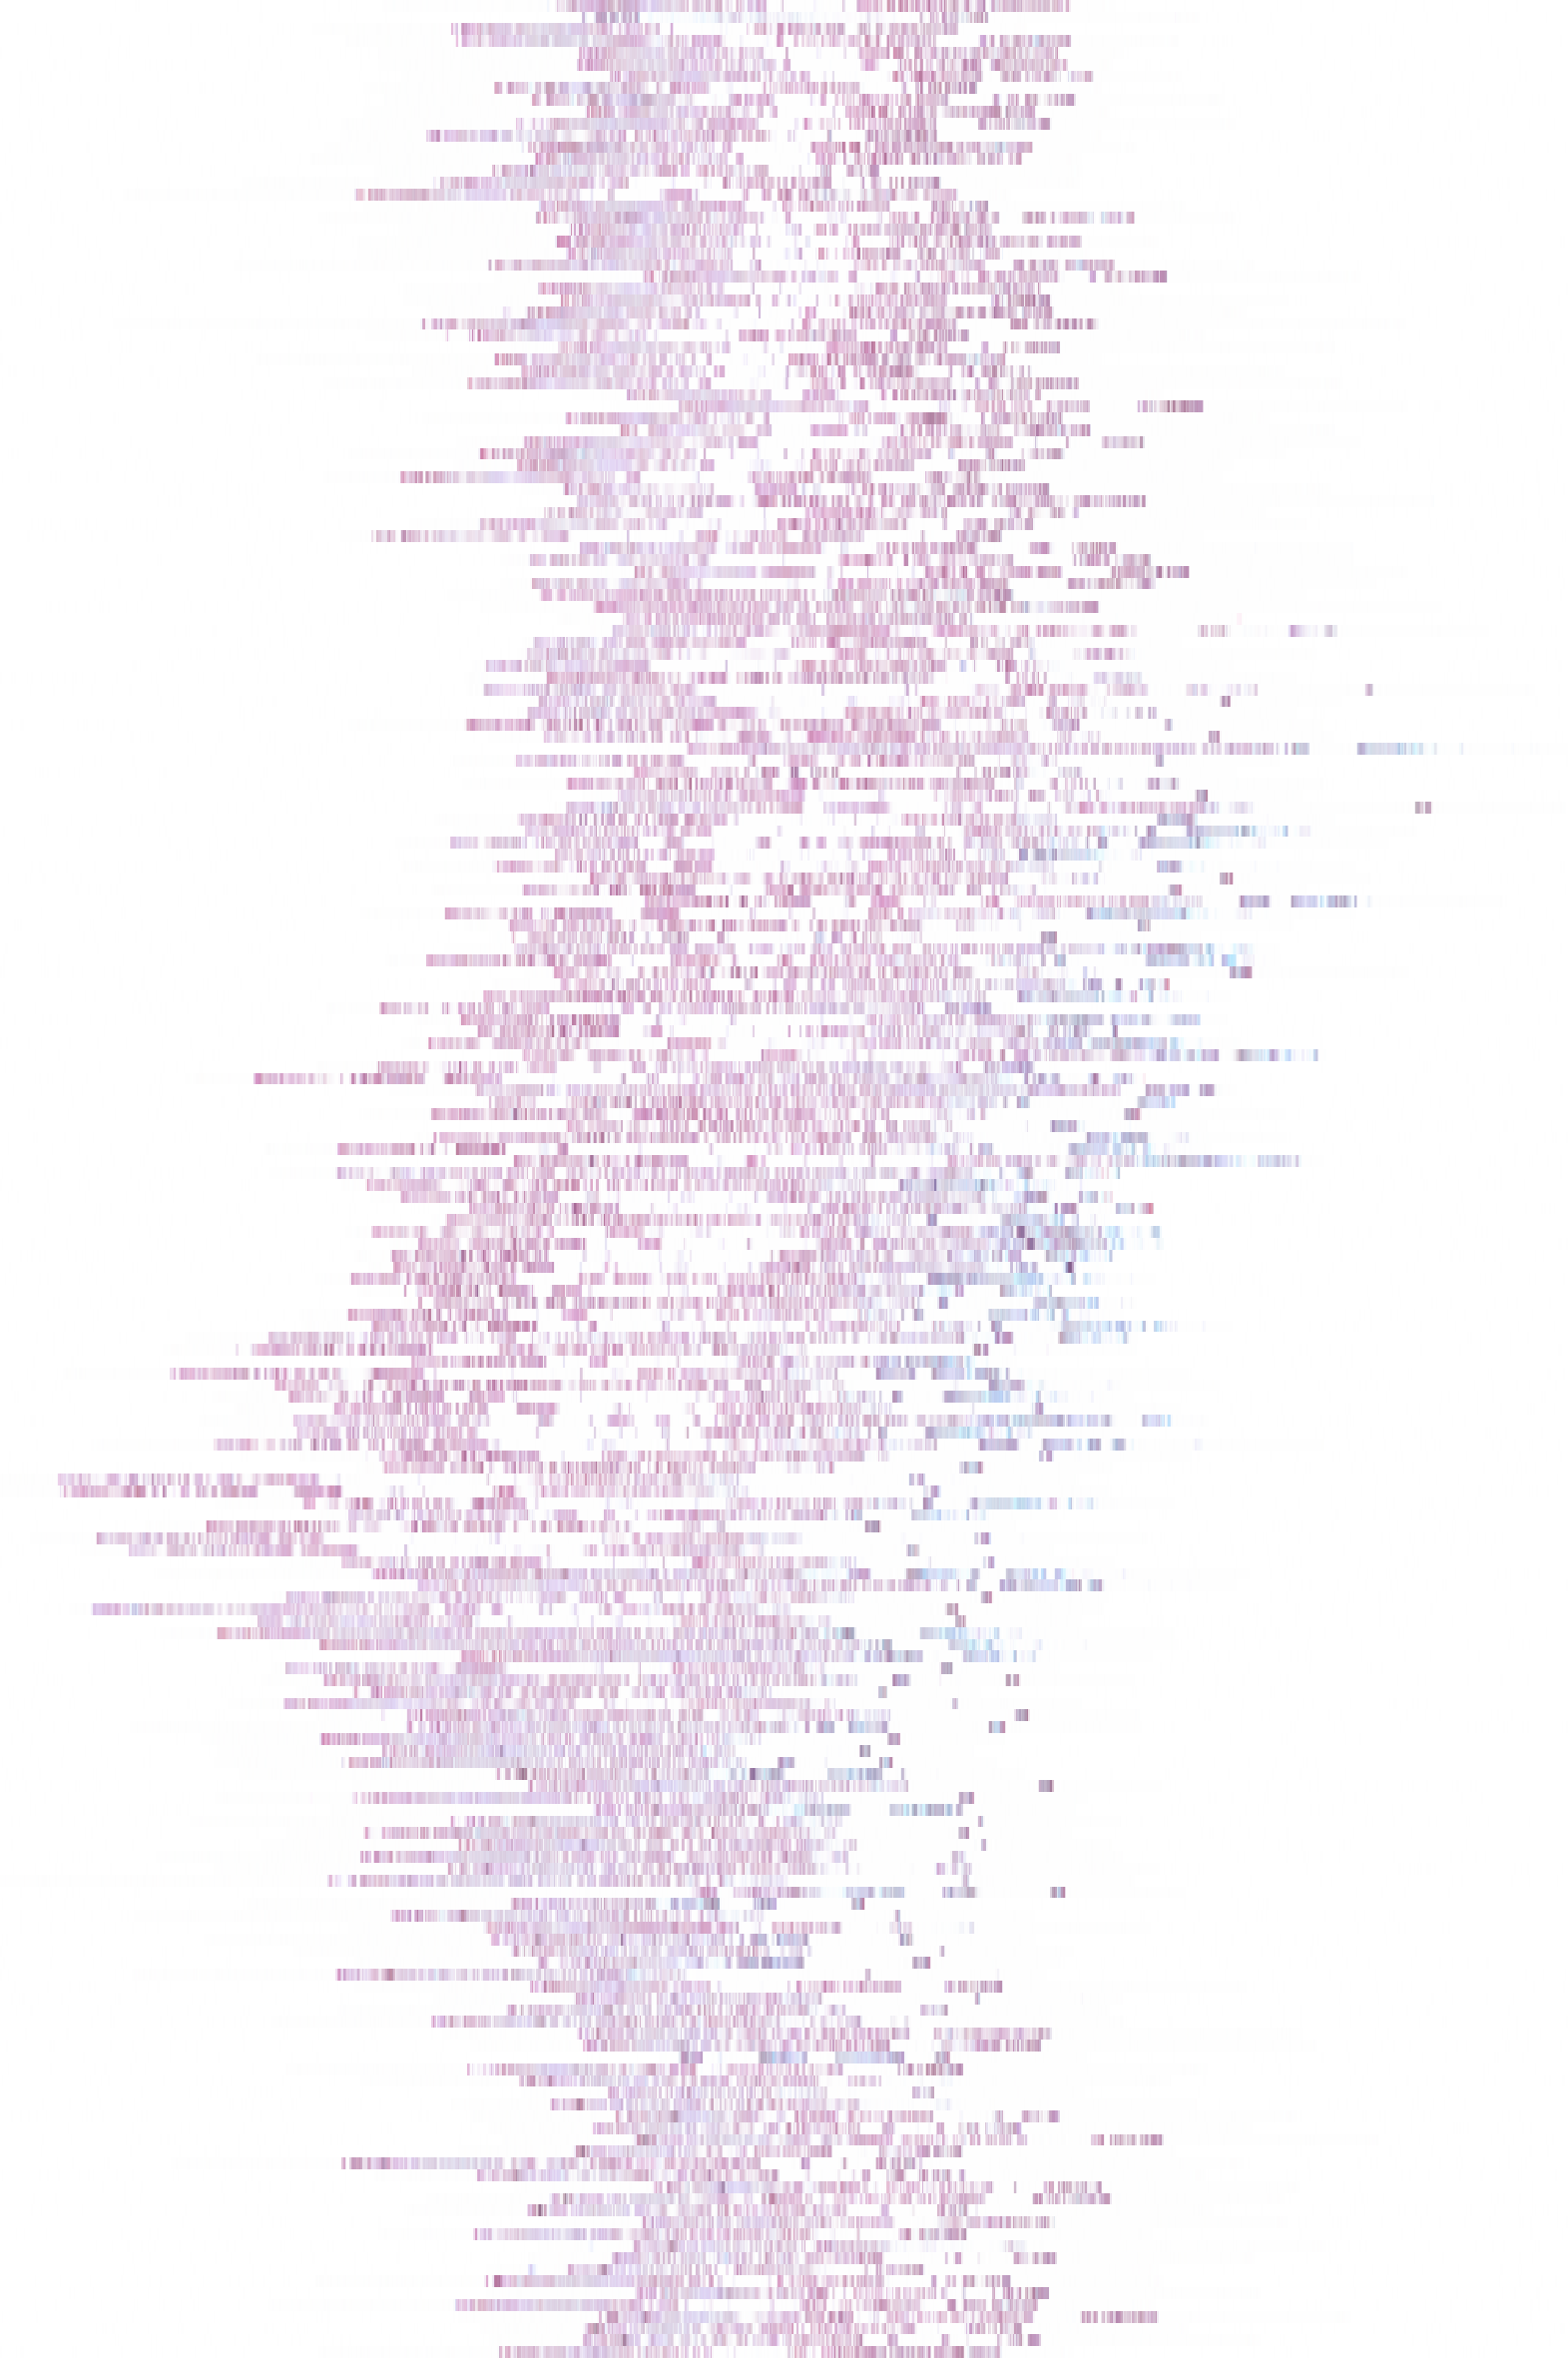
\includegraphics[width=1.1in]{2_methods/Figs/cross_section_0}\label{fig:synthetic_cross_section_0}}
    \subfloat[]{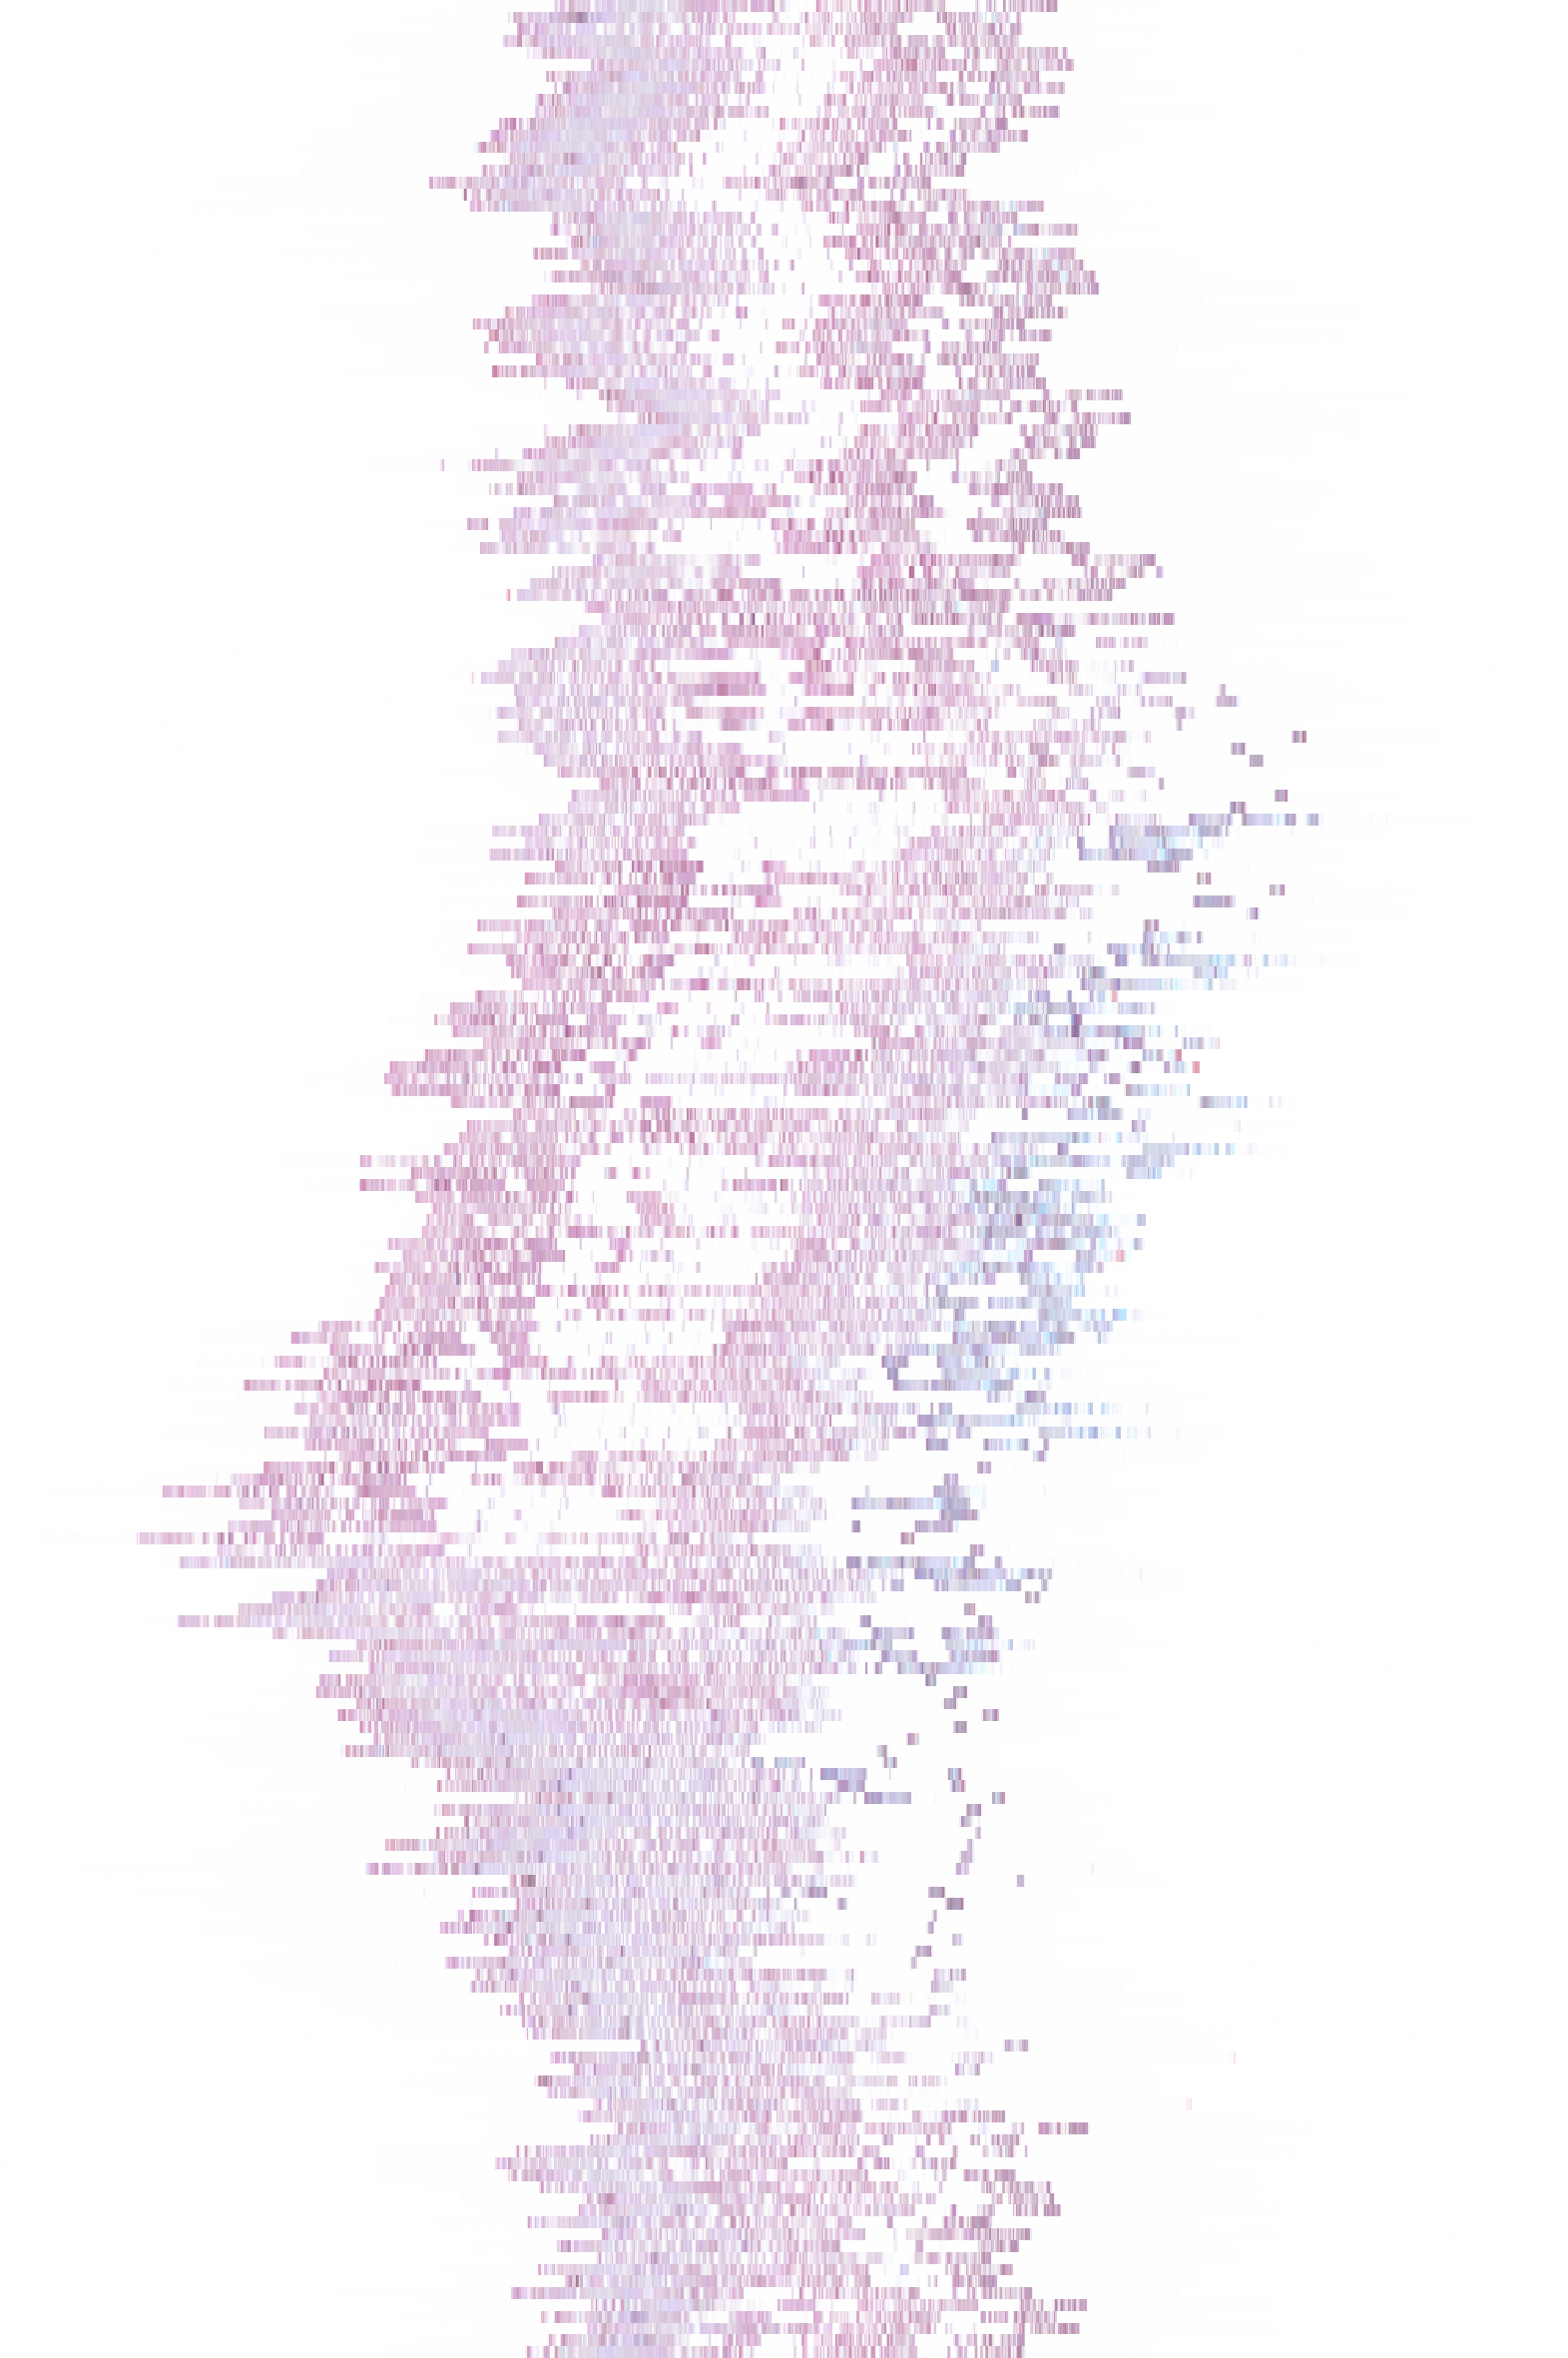
\includegraphics[width=1.1in]{2_methods/Figs/cross_section_1}}
    \subfloat[]{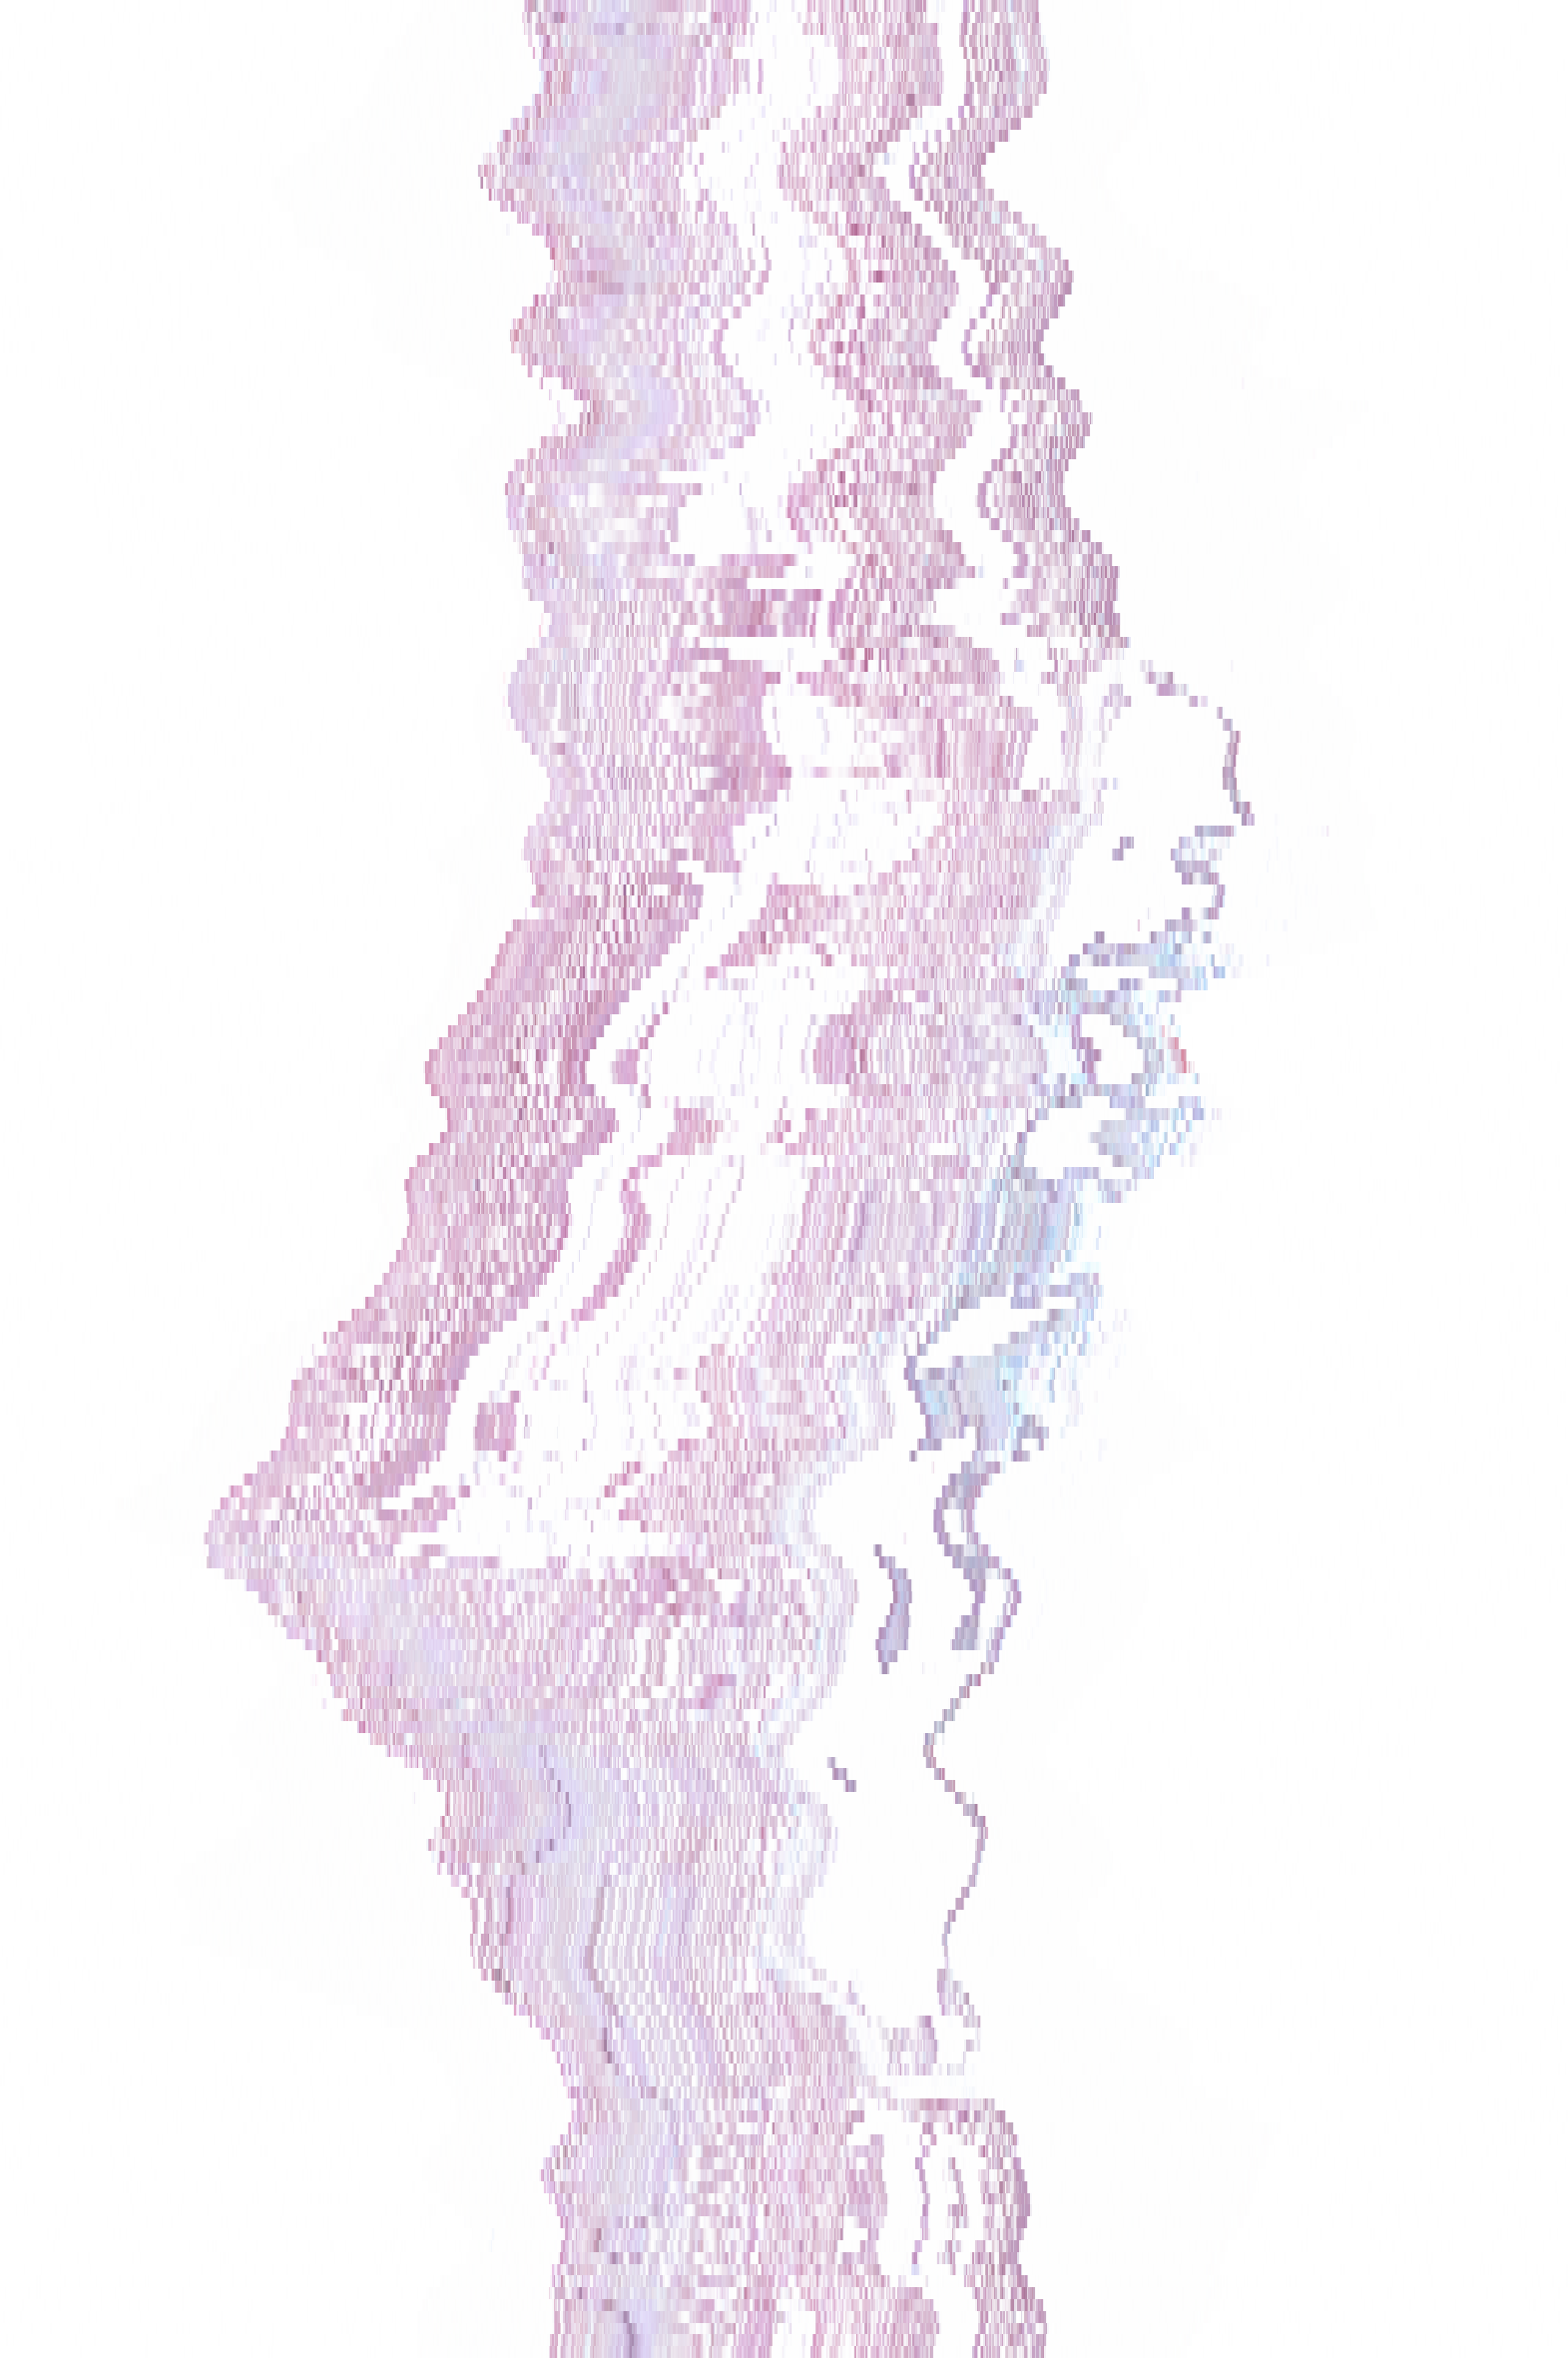
\includegraphics[width=1.1in]{2_methods/Figs/cross_section_7}}\\
    \subfloat[]{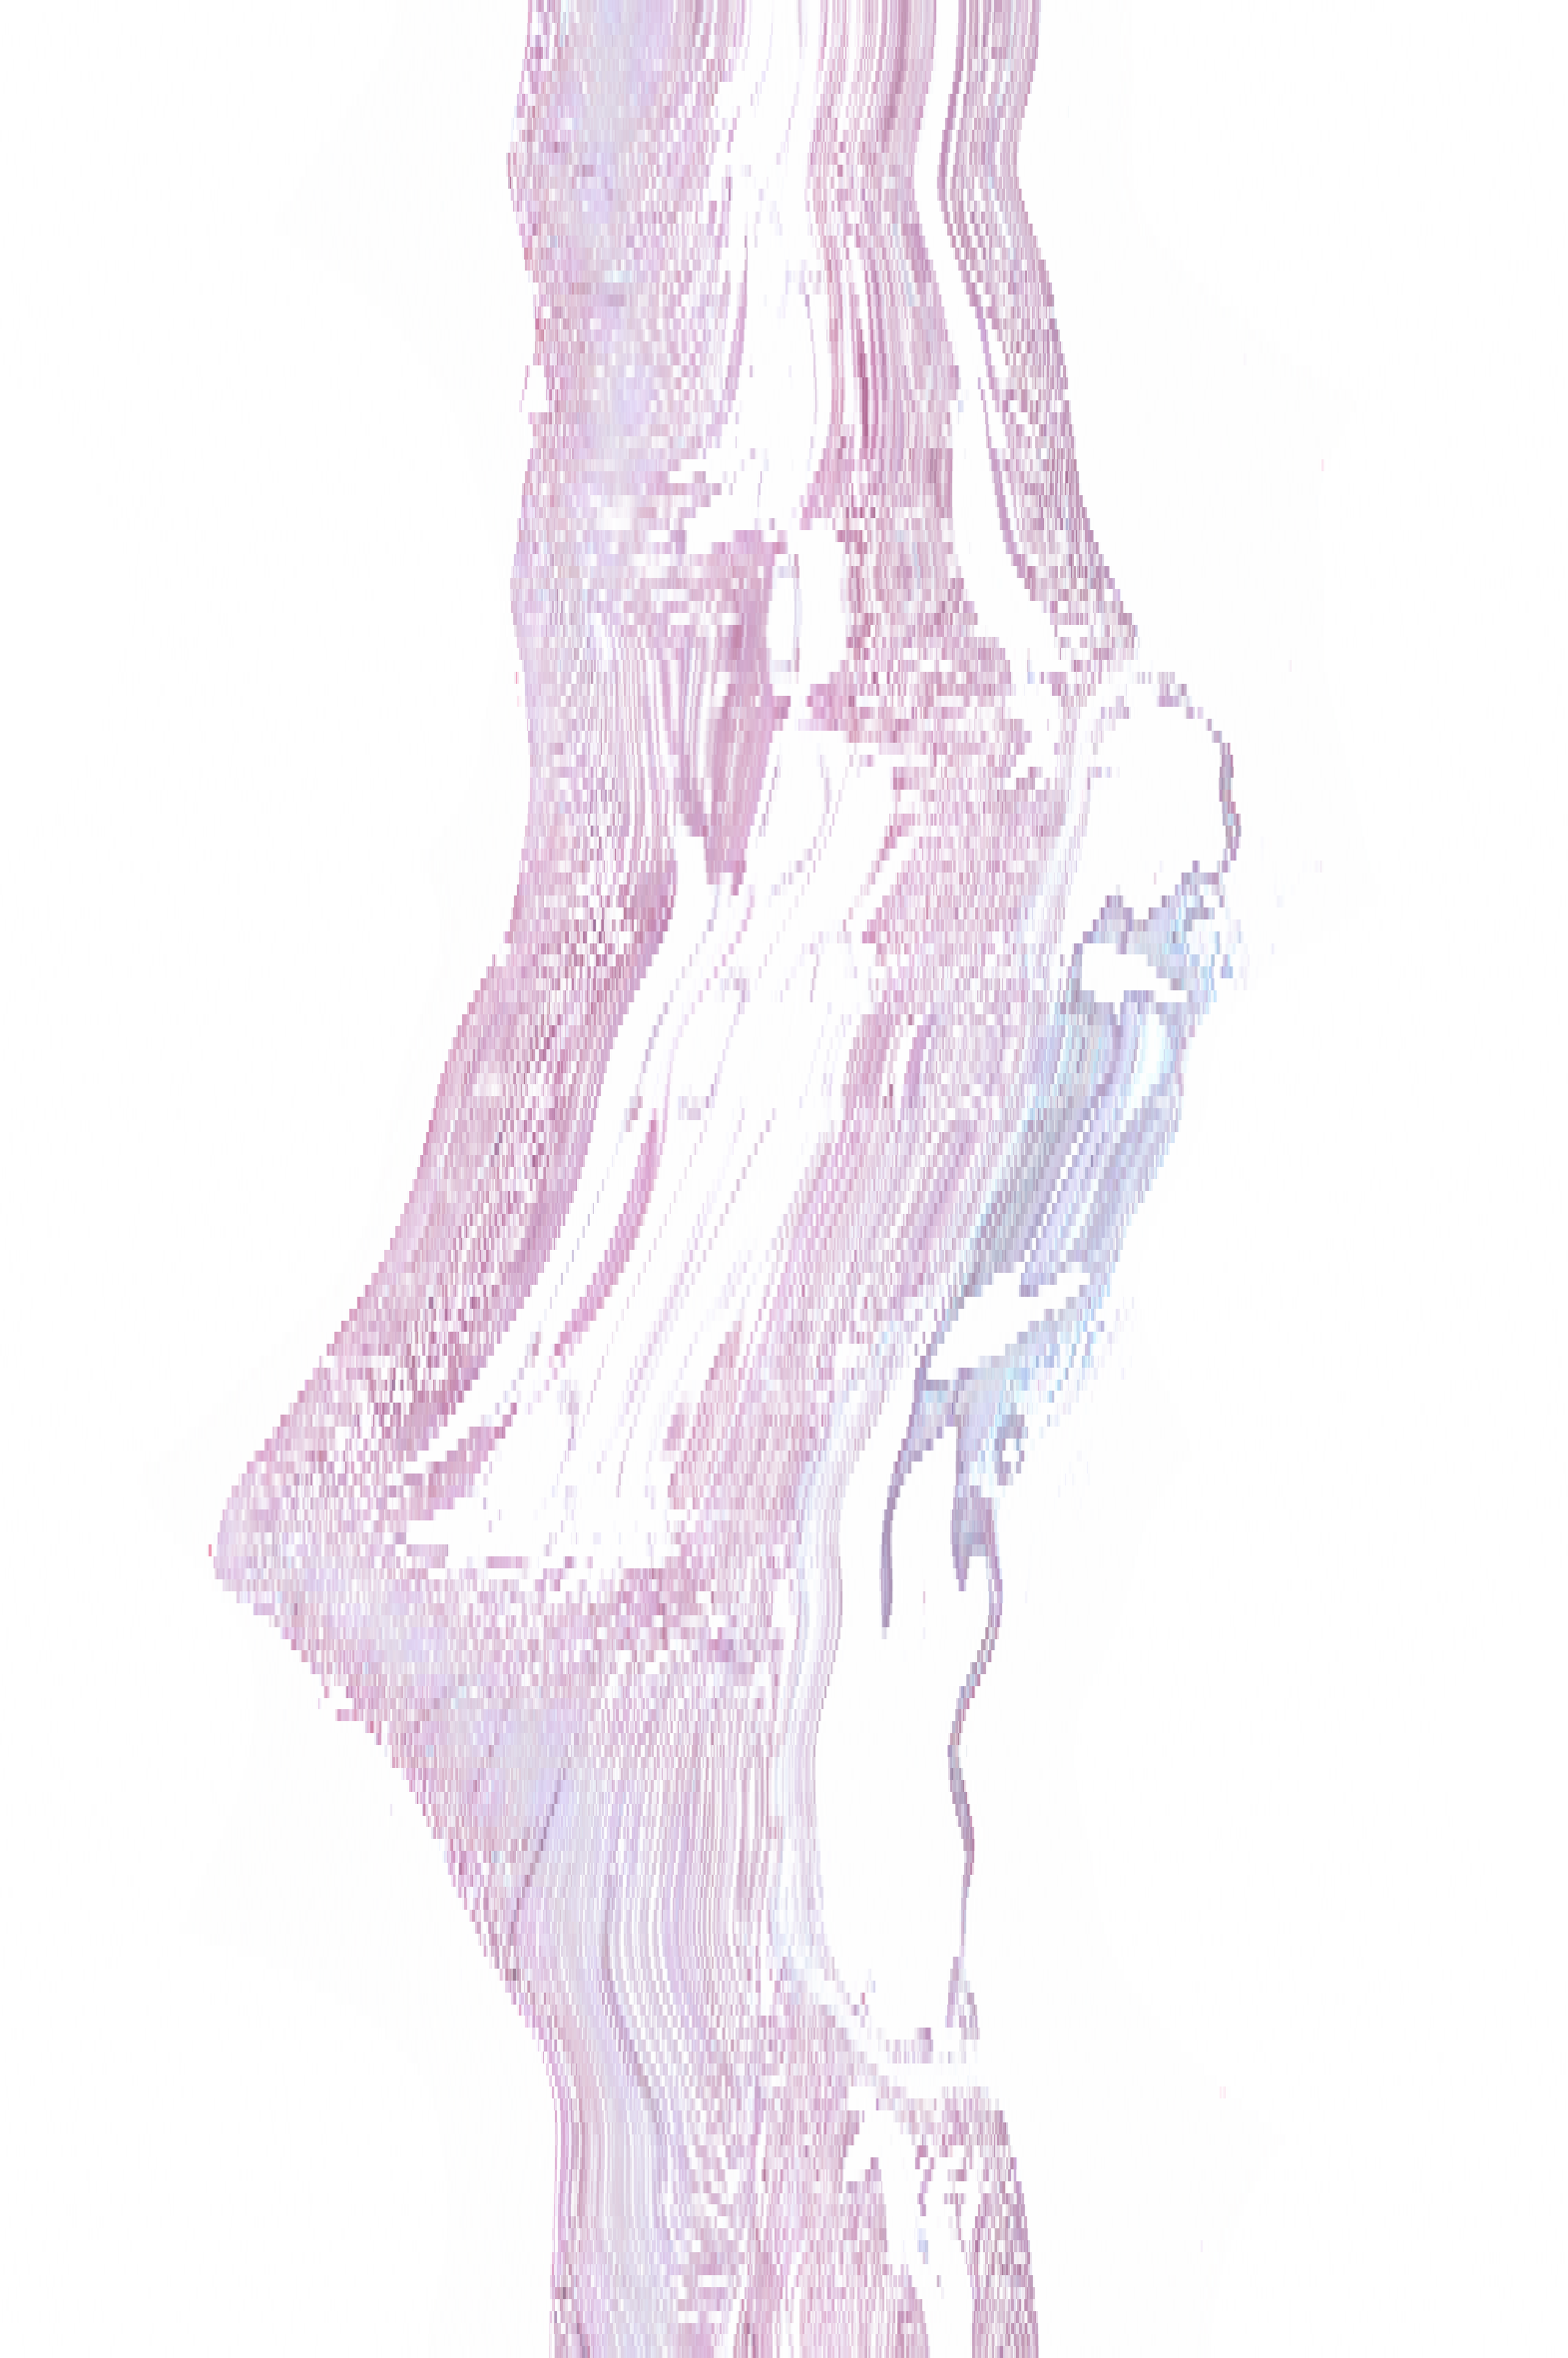
\includegraphics[width=1.1in]{2_methods/Figs/cross_section_40}}
    \subfloat[]{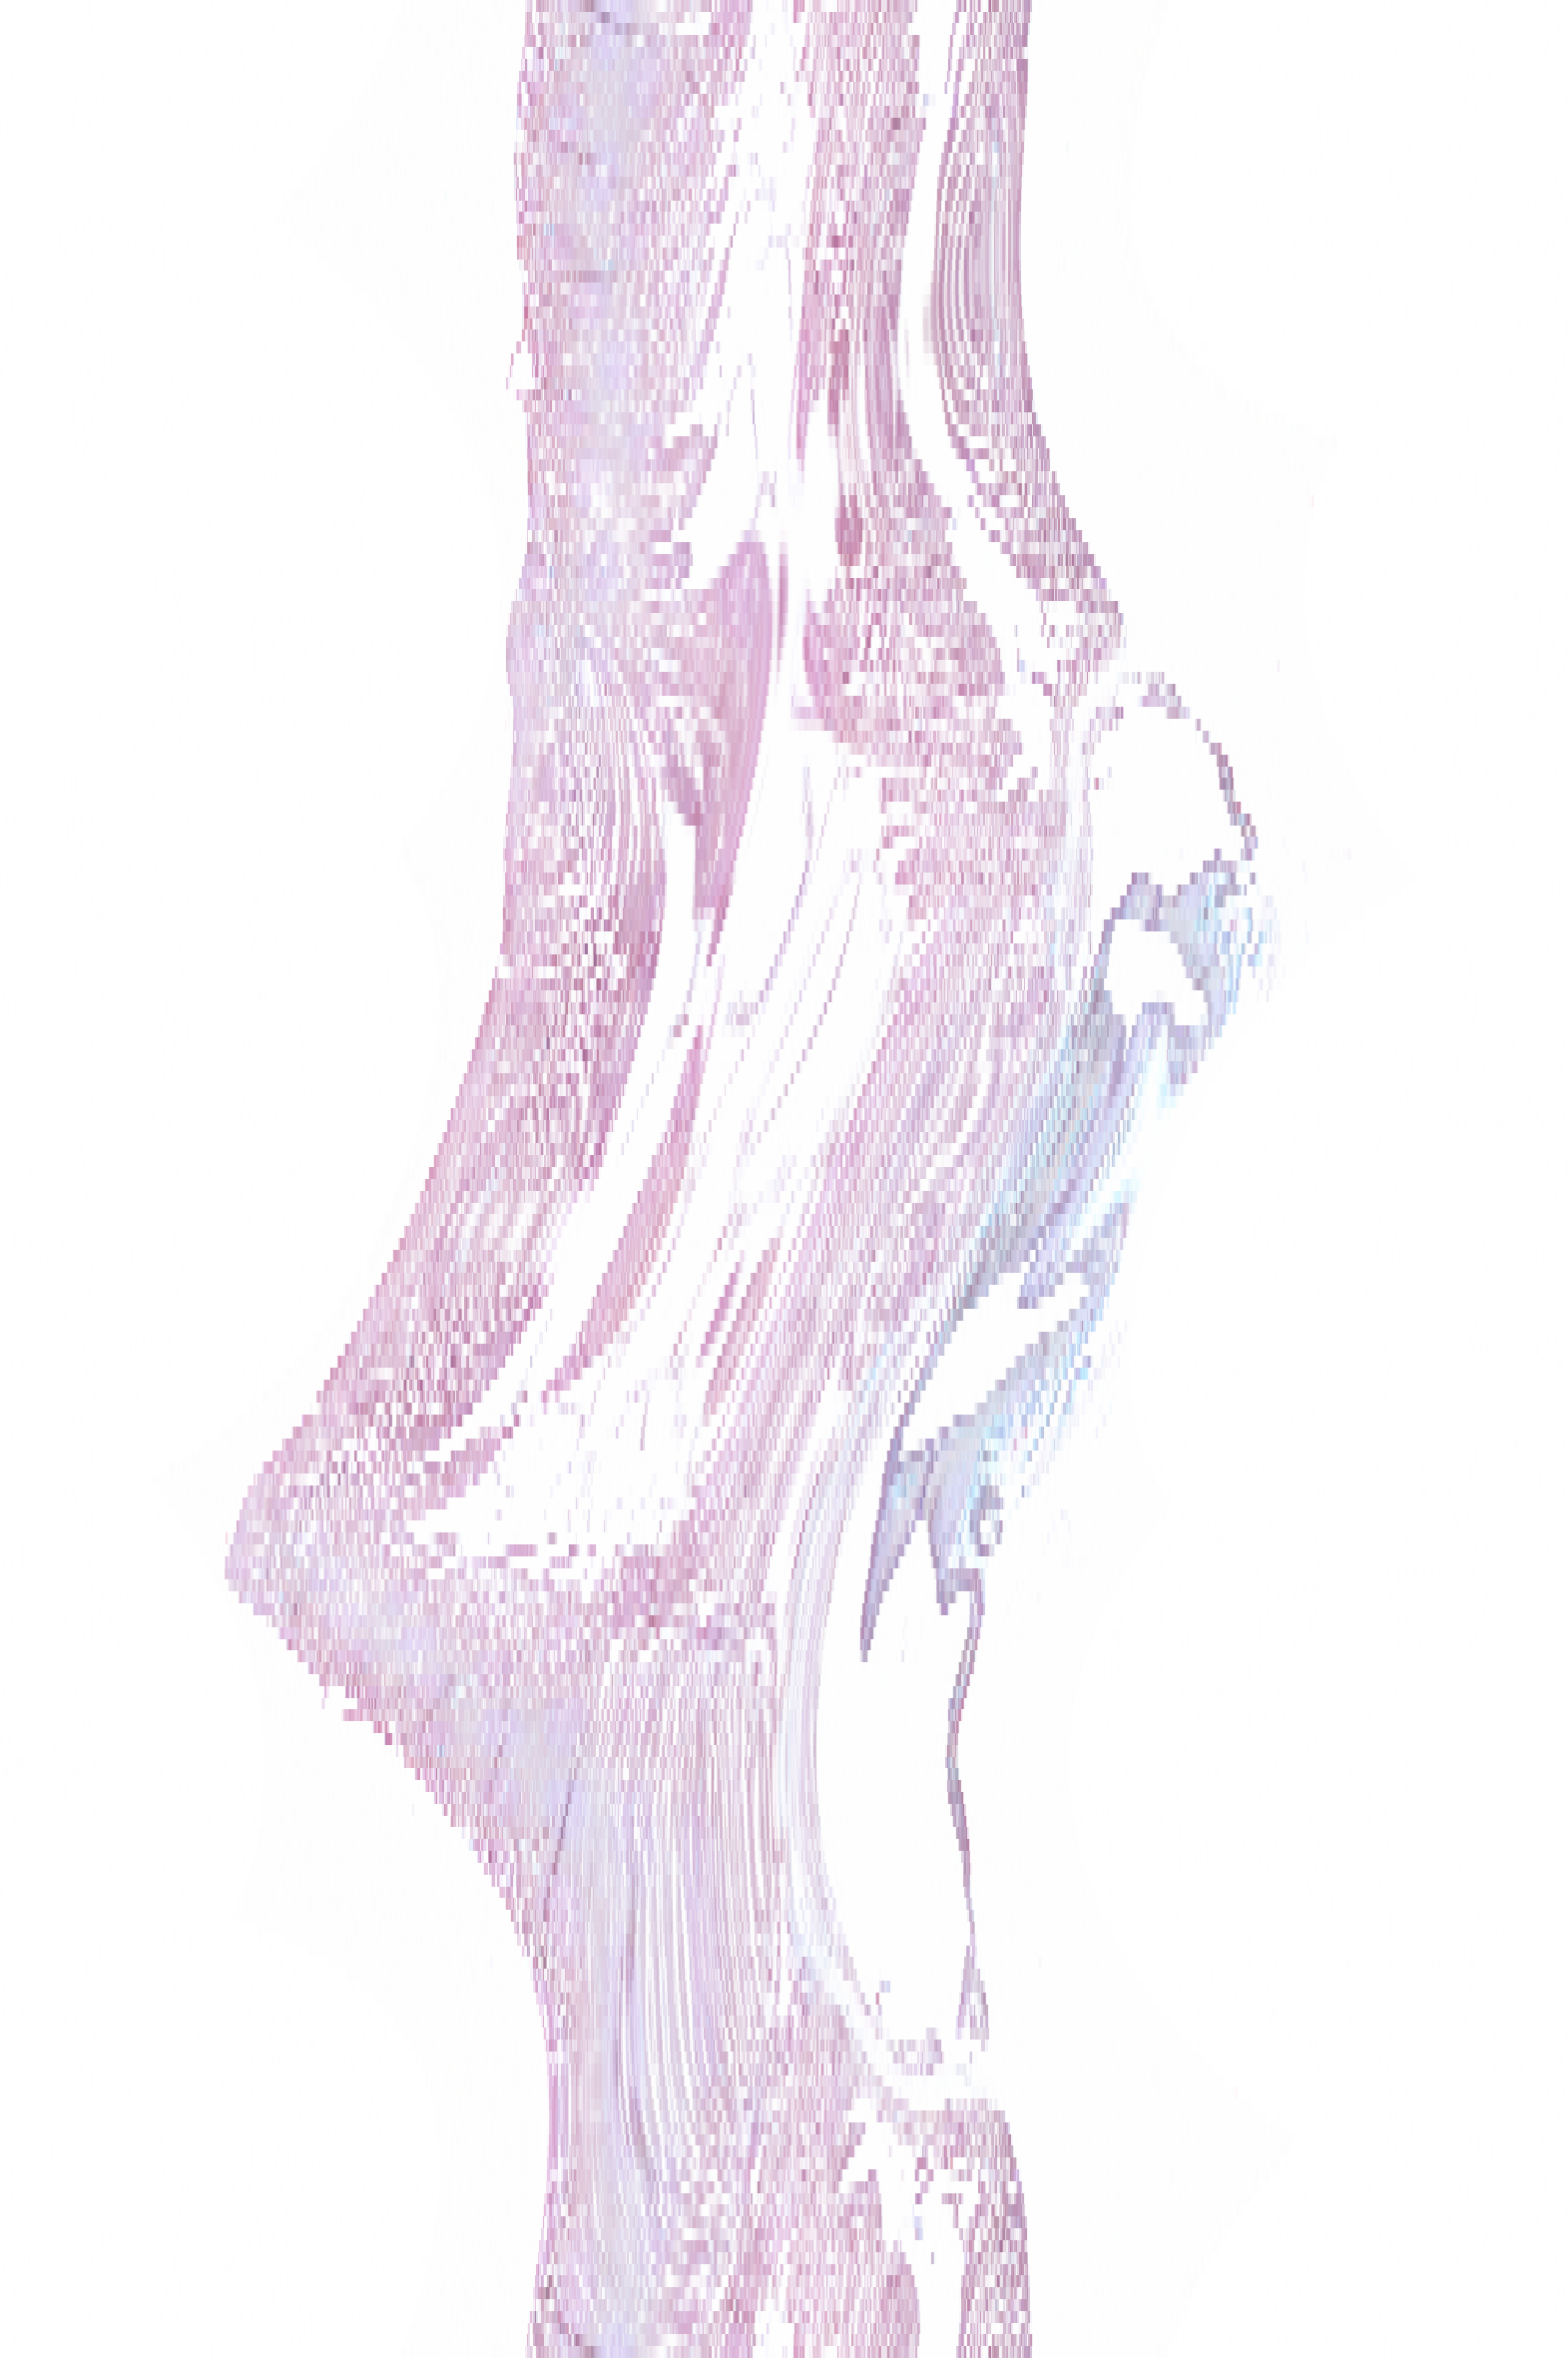
\includegraphics[width=1.1in]{2_methods/Figs/cross_section_perfect}}
    \subfloat[]{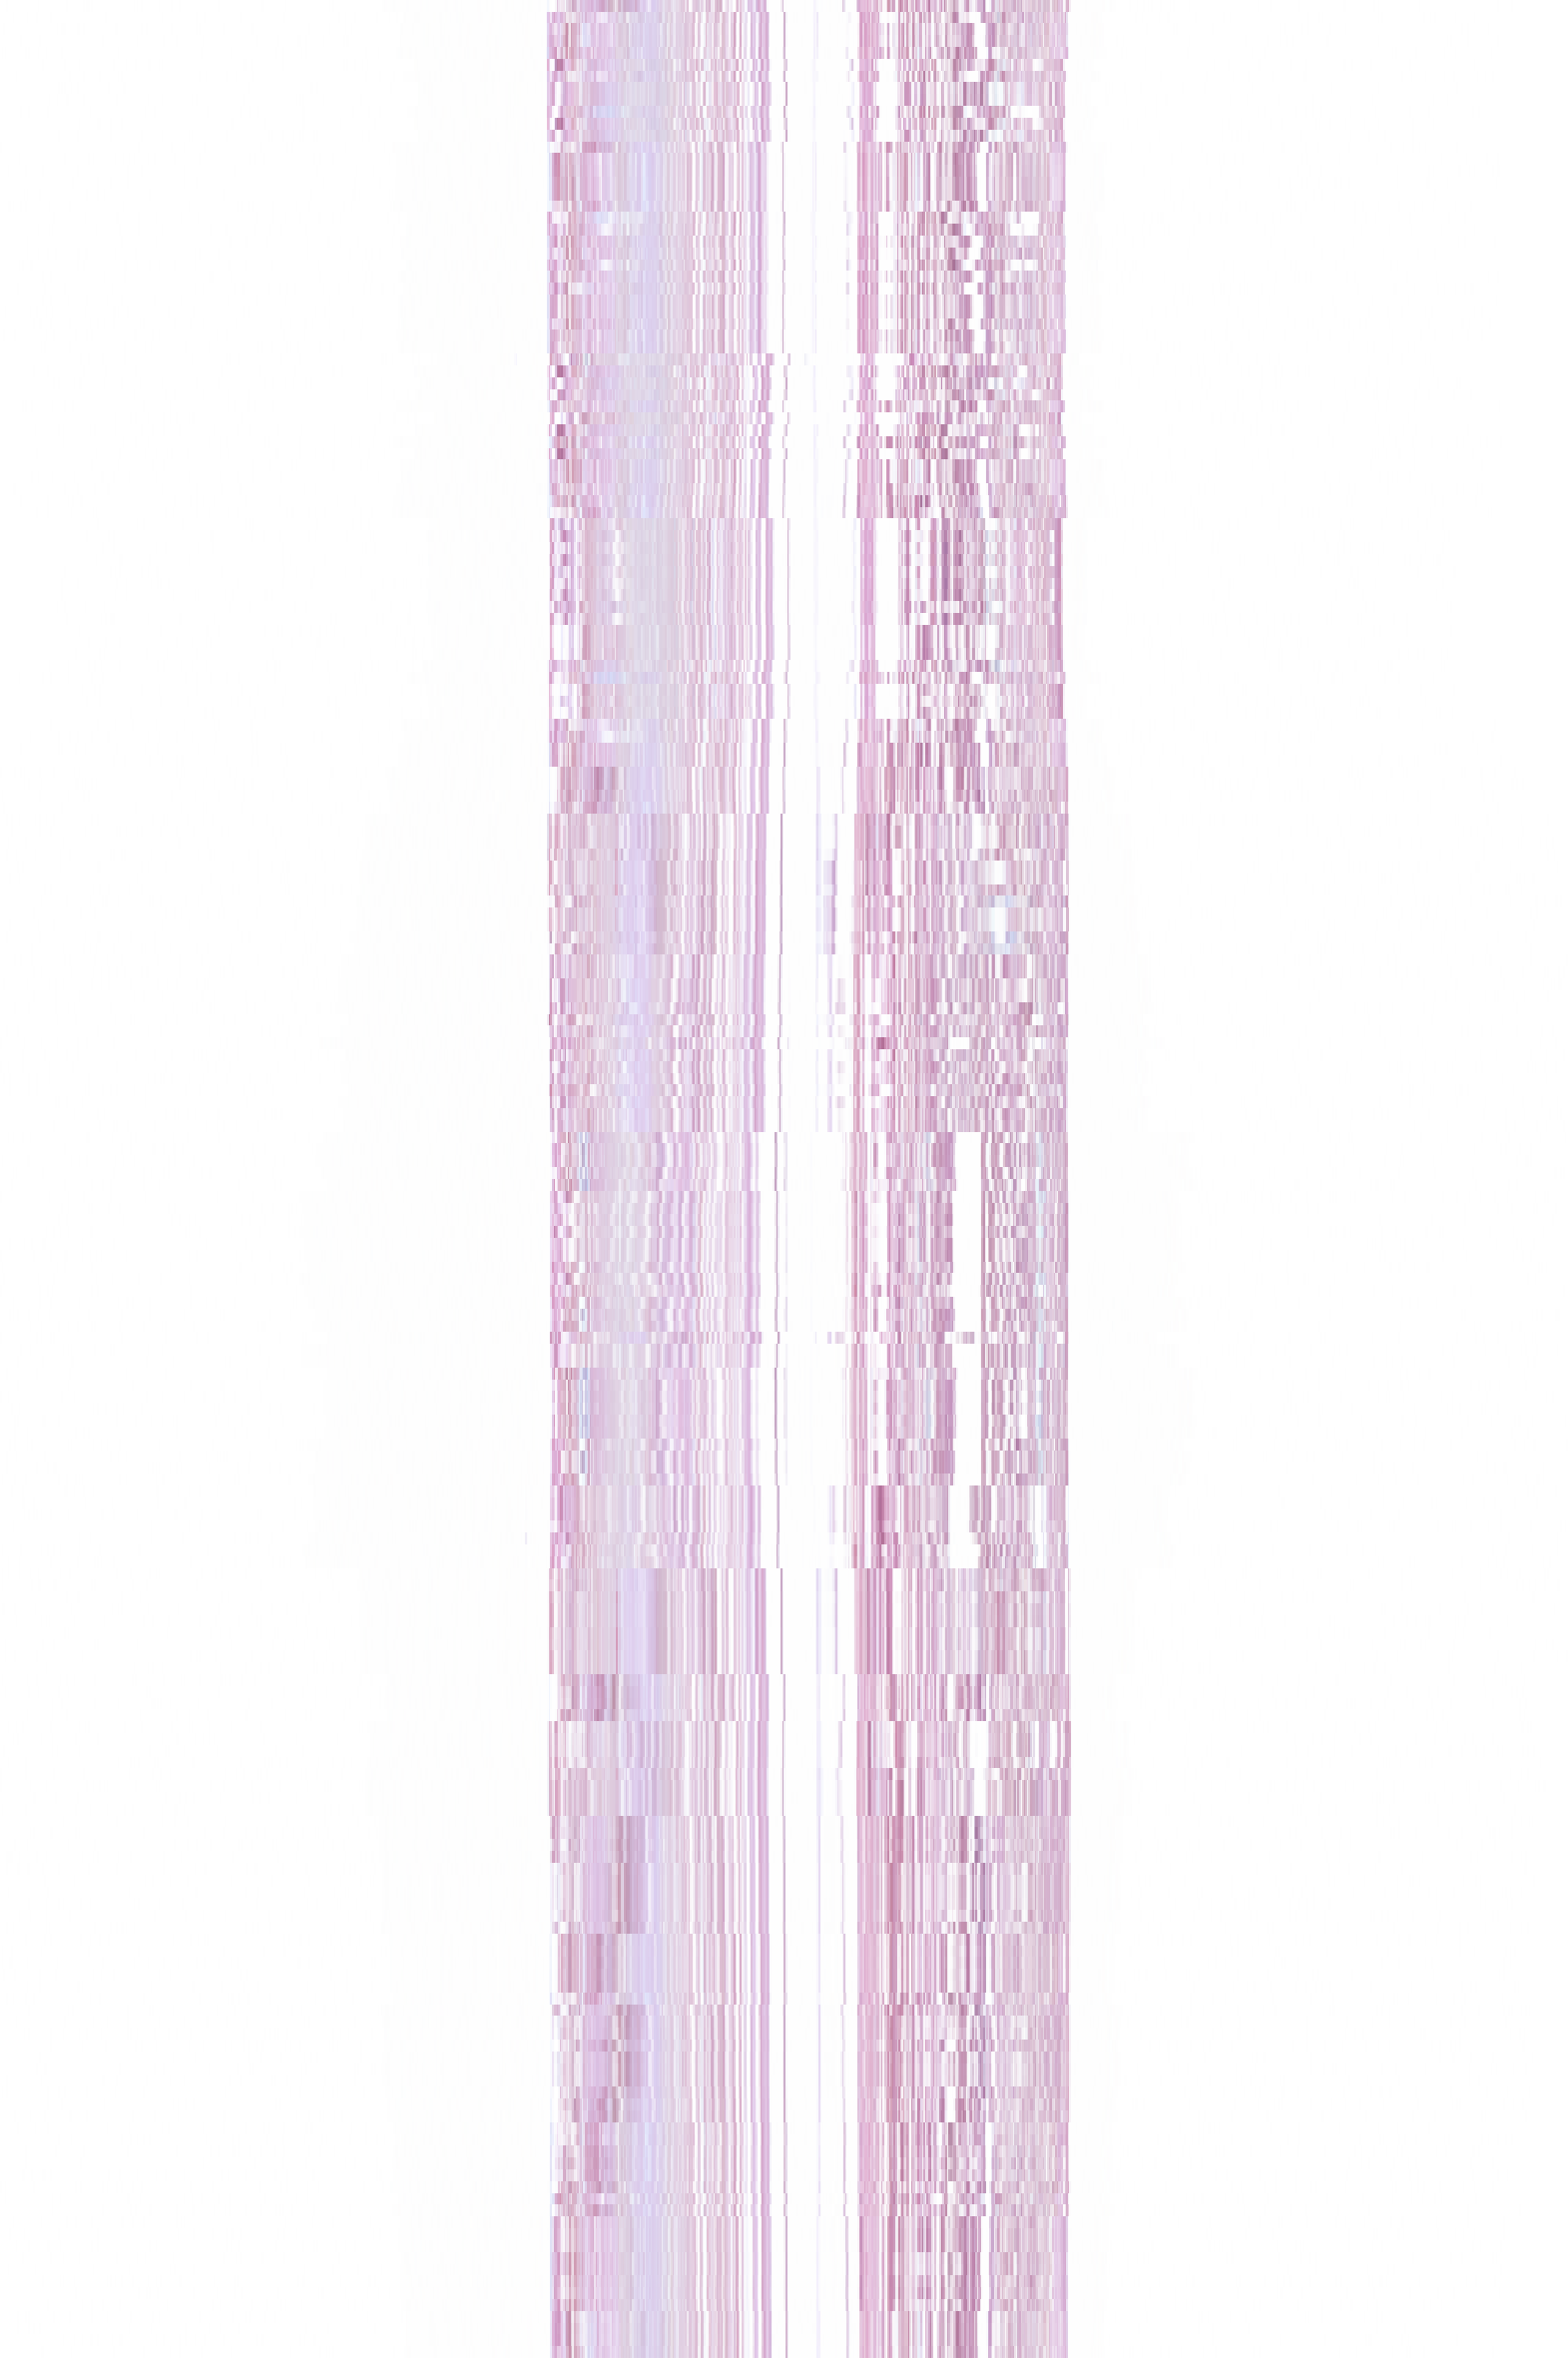
\includegraphics[width=1.1in]{2_methods/Figs/cross_section_banana}}
    \caption{Cross-sections of the synthetic volume (a) before TDS, (b) after 1 iteration, (c) after 7 iterations and (d) after 40 iterations, with (e) a cross-section of the unperturbed volume as a reference. (f) is the cross-section of a serially registered volume.}
    \label{fig:synthetic_cross_sections}
  \end{figure}
  The central cross-sections perpendicular to the x-axes are exhibited in Figure~\ref{fig:synthetic_cross_sections}. Cross-section (a) is of the original unsmoothed noisy volume, and (e) of the volume before noise was added. Three images are sandwiched by these two extremes, of sections smoothed 1, 7 and 40 times. The smoothing performs extremely well on two fronts. By iteration 40, a smooth, continuous section with the appearance of an original histology slice has been recovered from an unrecognisably noisy volume. Secondly and crucially, the underlying geometry of the tissue has been preserved, and the sections appear very similar to the ground truth sections before the noise had been added. Contrastingly, the banana effect is clear from (f), which has lost virtually all of the underlying sinusoidal signal.
  
  \begin{figure}[!t]
    \centering
    \subfloat[]{\includegraphics[width=1.1in]{2_methods/Figs/whole_surface_0}}
    \subfloat[]{\includegraphics[width=1.1in]{2_methods/Figs/whole_surface_1}}
    \subfloat[]{\includegraphics[width=1.1in]{2_methods/Figs/whole_surface_7}}\\
    \subfloat[]{\includegraphics[width=1.1in]{2_methods/Figs/whole_surface_40}}
    \subfloat[]{\includegraphics[width=1.1in]{2_methods/Figs/whole_surface_banana}}
    \caption{Contours of the perturbed synthetic volumes in red before TDS (a), and after 1 (b), 7 (c) and 40 (d) iterations, overlayed with the unperturbed volume in green. A contour of the serially registered volume in green is shown in (e).}
    \label{fig:synthetic_contours}
  \end{figure}
  The nature of the 3-D geometry of the volumes --- the rotation and translation signals, and the transformational noise --- is most clearly understood from the segmentation volume isosurfaces in Figure~\ref{fig:synthetic_contours}. Each of the 4 levels of smoothing depicted by Figure~\ref{fig:synthetic_cross_sections} are overlayed in red with the unperturbed volume in green. Again, the smoothing brings the noisy volume much more closely in line with the ground truth, with the largest effect on the higher frequencies of noise. The conservation of the underlying structure is most evident in Figure~\ref{fig:synthetic_contours}~(d), where the red isosurface deviates almost imperceptibly from the green. The surface of (e) is greatly more discontinous than the red surface of (d), each slice pair having only been coregistered once.

  % Evolution of error from ground truth
  \begin{figure}[!t]
    \subfloat[]{\includegraphics[width=1.7in]{2_methods/Figs/absolute_errors_2d}\label{fig:absolute_errors_2d}}
    \subfloat[]{\includegraphics[width=1.7in]{2_methods/Figs/relative_errors_2d}\label{fig:relative_errors_2d}}
    \caption{Slicewise absolute (a) and relative (b) mean pixel Euclidean distance errors of the initial (blue), final (green) and sequentially registered (red) synthetic volumes. The absolute volumewise means are 1393, 271.6 and 4204 and the relative means are 1929, 37.94 and 134.8, for the initial, final and sequential volumes respectively.}
    \label{fig:synthetic_errors}
  \end{figure}
  Figure~\ref{fig:synthetic_errors}~(a) graphs the mean Euclidean distance of the pixels within a segmentation of the slice from their unperturbed ground truth position, before and after smoothing, and after serial registration. Almost ubiquitously, the metric is greatly reduced after TDS, evidence that each slice is much more closely aligned to its true position. The overall sinusoidal nature of the serial registration is of course due to the loss of the ground truth morphology. The error after TDS is prominently the smoothest of the three lines, reflecting the continuity of the volume and the preferential damping of the high frequency spectrum.

  Mean relative Euclidean errors in Figure~\ref{fig:synthetic_errors}~(b) --- distances of pixels in slice $n+1$ from their ground truth positions, both measured from the respective reference frames of slice $n$ --- are cleanly separated on a log scale. The same spectral patterns are observed. Volumewise absolute error is reduced by a factor of 5.1 and relative error by 50 after TDS.

  \subsection{Block Face Registration of Histology} % (fold)
  \label{sub:block_face_registration_of_histology}
  % figure of full cross-sections, unregistered, banana registered and lo-res registered, with lores equivalent slice
  \begin{figure}[!t]
    \centering
    \subfloat[]{\includegraphics[height=1.2in]{3_results/Figs/LoRes_1_287}}
    \subfloat[]{\includegraphics[height=1.2in]{3_results/Figs/geometric_1_287}}\\
    \subfloat[]{\includegraphics[height=1.2in]{3_results/Figs/affine_1_287}}
    \subfloat[]{\includegraphics[height=1.2in]{3_results/Figs/banana_1_301}}
    \caption{Equivalent cross-sections of (a) the block face volume, (b) the histology slices before registration, aligned to their common geometrical centre, (c) the block face-registered histology slices and (d) the sequentially registered slices with no reference volume.}
    \label{fig:block_face_registration}
  \end{figure}
  Cross-sections of block face, unregistered, block face-registered and serially registered volumes are presented in Figure~\ref{fig:block_face_registration}. We achieve a reasonable large-scale alignment of the great majority of histological slices to form a consistent tissue volume, as is clear from a comparison of Figure~\ref{fig:block_face_registration} (a) and (c). Yet we are left with several limitations of the block face technique. Striations are visible in (a) due to discrete changes in the positioning and intensity of illumination between block face image acquisitions. These changes propagate to the final block face registration result. At 26.6 $\mu$m, the in-plane resolution of the reference images is 24 times coarser than that of the histology slices (evident in Figure~\ref{fig:raw_images}), precluding an alignment on the scale of cardiac microstructure. Small non-rigid deformations introduced during slicing and rehydration are particular to each slice, and could not be represented fully by the affine registration. Despite obtaining a result that was relatively close to the block face geometry, the overlap of pixel intensities between tissue and wax, and the interslice variability therein, leads to a noisy, jagged result that is not always at the global minimum.
  
  Even when constrained by a rigid transform, in many areas the slice-to-slice registration in Figure~\ref{fig:block_face_registration}~(d) is accurate enough that detailed tissue structure is clearly visible. Yet, just as the prism-like synthetic volume does not represent the oscillatory volume in Figure~\ref{fig:synthetic_contours}, the resulting geometry of the volume is quite unrelated to the ground truth of the block face volume.
  
  \subsection{TDS on Block Face-Registered Histology} % (fold)
  \label{sub:tds_on_block_face_registered_histology}
  % figure of regional cross-section before smoothing, after global smoothing and after regional smoothing
  \begin{figure}[!t]
    \centering
    \subfloat[]{\includegraphics[width=3.4in]{3_results/Figs/unsmoothed_vessel_1_2125}}\\
    \subfloat[]{\includegraphics[width=3.4in]{3_results/Figs/globally_smoothed_vessel_1_2125}}\\
    \subfloat[]{\includegraphics[width=3.4in]{3_results/Figs/regionally_smoothed_vessel_1_2125}}
    \caption{Central cross sections of the region around an epicardial vessel. Cross-sections are compared before smoothing, after global smoothing and after smoothing applied to this region. The blue arrow highlights blue-stained interstitial tissue around vessels, the green arrow epicardial vessels and the yellow arrow enhanced sheet structure.}
    \label{fig:vessel_sections}
  \end{figure}
  An unmistakable improvement in coherence is observed after global smoothing, exemplified in Figure~\ref{fig:vessel_sections}~(a) and (b); edges are smoother and waving sheet structure emerges, previously indistinguishable beyond the high-frequency zig-zagging noise. The outer walls are several orders of magnitude less noisy, and internal vessel walls are much more coherent. A regional registration around an epicardial vessel yields even further improvement in (c), when at this smaller scale, curvature and distortions not represented by an affine transformation become less significant.

  % figure of vessel and surface contour before smoothing and after regional smoothing
  \begin{figure*}[!t]
    \centerline{\subfloat[]{\includegraphics[width=2.4in]{3_results/Figs/unsmoothed_segmentation}} \hfil
    \subfloat[]{\includegraphics[width=2.4in]{3_results/Figs/globally_smoothed_segmentation}} \hfil
    \subfloat[]{\includegraphics[width=2.4in]{3_results/Figs/locally_smoothed_segmentation}}}
    \caption{Surface contours of segmentations of vasculature (red) and epicardium (green) in the region around an epicardial vessel from Figure~\ref{fig:vessel_sections}, from the unsmoothed, globally smoothed and locally smoothed volumes.}
    \label{fig:region_segmentations}
  \end{figure*} 
  In Figure~\ref{fig:region_segmentations}, progressive enhancement in coherence is visible from the back cross-section, the vessel surface and the pericardial surface, from (a) to (b) and then to (c); the contours in (c) are almost totally smooth, with only the inherent stepping of each individual histology slice visible. In particular, the disturbance near the top of the largest vessel in (b) has been smoothed in (c). Original adjacent slice aberrations in (a) reached ~450$\mu$m. Contrastingly in (c), the relative registration error is reduced below the diameter of even the smallest vessels, by inspection less than 5$\mu$m in the large majority of cases - smaller than the width of a single myocyte. Resultingly, with each of the two smoothing procedures, more of the smaller vasculature has become connected to the main vessel and has been segmented.
    
  % figure of vessel and surface contour before smoothing and after regional smoothing
  \begin{figure}[!t]
    \centering
    \includegraphics[width=3.4in]{3_results/Figs/vessel_overlay}
    \caption{An overlay of the three vessel segmentations from Figure~\ref{fig:region_segmentations}. The unsmoothed vessel is shaded in red, the globally smoothed vessel in amber and the regionally smoothed vessel in green.}
    \label{fig:vessel_segmentations}
  \end{figure} 
      We see the combined results of all three vascular segmentations in Figure~\ref{fig:vessel_segmentations}. From this view through the pericardium, the striking continuity of the green surface is most apparent. The overall shape of the green vessel precisely intersects the disconnected set of red discs, demonstrating that the underlying vessel geometry has been recovered with remarkable accuracy. Again it is clear that the reduction in error below the diameter of the smallest vessels has facilitated their segmentation, with several thin green dendritic structures reaching up into the top left of the figure.  
  % subsection regional_diffusion (end)
% section results (end)
